\documentclass{article}


% if you need to pass options to natbib, use, e.g.:
%     \PassOptionsToPackage{numbers, compress}{natbib}
% before loading neurips_2023


% ready for submission
\usepackage[final]{neurips_2023}
\usepackage{graphicx}
\usepackage{subcaption}

% to compile a preprint version, e.g., for submission to arXiv, add add the
% [preprint] option:
%     \usepackage[preprint]{neurips_2023}


% to compile a camera-ready version, add the [final] option, e.g.:
%     \usepackage[final]{neurips_2023}


% to avoid loading the natbib package, add option nonatbib:
%    \usepackage[nonatbib]{neurips_2023}


\usepackage[utf8]{inputenc} % allow utf-8 input
\usepackage[T1]{fontenc}    % use 8-bit T1 fonts
\usepackage{hyperref}       % hyperlinks
\usepackage{url}            % simple URL typesetting
\usepackage{booktabs}       % professional-quality tables
\usepackage{amsfonts}       % blackboard math symbols
\usepackage{nicefrac}       % compact symbols for 1/2, etc.
\usepackage{microtype}      % microtypography
\usepackage{xcolor}         % colors
\usepackage{graphicx}


\title{Medical Image Segmentation With Retinal Image Data }


% The \author macro works with any number of authors. There are two commands
% used to separate the names and addresses of multiple authors: \And and \AND.
%
% Using \And between authors leaves it to LaTeX to determine where to break the
% lines. Using \AND forces a line break at that point. So, if LaTeX puts 3 of 4
% authors names on the first line, and the last on the second line, try using
% \AND instead of \And before the third author name.


\author{%
  \thanks{} \\
  Department of Computer Science and Engineering\\
  Indraprastha Institute of Information Techonology\\
  Authors\\
  \texttt{Junaid Fayaz Lone, Mohit Bhardwaj }\\
  \texttt{Paras Dhiman , Arnav Agarwal , Shubham Kumar } 
  }
  % examples of more authors
  % \And
  % Coauthor \\
  % Affiliation \\
  % Address \\
  % \texttt{email} \\
  % \AND
  % Coauthor \\
  % Affiliation \\
  % Address \\
  % \texttt{email} \\
  % \And
  % Coauthor \\
  % Affiliation \\
  % Address \\
  % \texttt{email} \\
  % \And
  % Coauthor \\
  % Affiliation \\
  % Address \\
  % \texttt{email} \\
}


\begin{document}


\maketitle

\begin{abstract}


The exponential growth of digital images has spurred a compelling shift towards the study of computer vision in various fields in medical diagnosis. One area of particular interest is the analysis of retinal vasculature. This information is used in medical diagnosis and exploration of various conditions, including hypertension, diabetic retinopathy, cataracts, glaucoma, and cardiovascular diseases. We have prepared an SVM based model for the segmentation of retinal images and identification of blood vessels, after drawing inferences from existing research. 


\end{abstract}

\section{Exploratory Data Analysis}
There are a total of 28 images with 14 being for the left eye and 14 for the right eye. All images are circular with a black background. There is a iris clearly visible in the center of the optical disc.The blood vessels are also visible in the optical disc.

All images have the same size of 960x999 pixels which is a total of 959040 pixels per image.

The mean pixel intensity across all pixels of all images is 54.79.As expected the variation is not significant across the two eyes.

Standard deviation of pixel intensities across the dataset is 73.64.

\subsection{Histogram Equalization}

Histogram Equalization is applied to all images, enhancing image contrast by redistributing pixel intensities.
\begin{figure}[h]
  \centering
  \includegraphics[width=0.8\textwidth]{check1.png}
  \caption{Illustration of Histogram Equalization Process}
  \label{fig:example}
\end{figure}
Interpretation:
Histogram Equalization(Figure 1) improves image contrast by making the intensity distribution more uniform. This can reveal hidden details and enhance visual quality, particularly in low-contrast images.Histogram equalization is essential for assessing and enhancing the quality of images. 

\subsection{Image Statistics}

\begin{figure}[h]
  \centering
  \includegraphics[width=0.8\textwidth]{check2.png}
  \caption{Pixel Intensity Histograms}
  \label{fig:example}
\end{figure}

An important EDA task is to show pixel intensity histograms(Figure 2). Further to build pixel intensity histograms, we first converts color images to grayscale, simplifying the analysis by focusing on single-channel intensity.


Another critical aspect of image Exploratory Data Analysis (EDA) is to calculate and visualize statistics for each image in the dataset. Our computations include mean pixel intensity, standard deviation, minimum intensity, and maximum intensity. These statistics serve to characterize the distribution and variability of pixel intensities in the images. Box plots are generated to visually represent the distribution of these statistics. 

The box plots(Figure-3) offer valuable insights into the distribution and variability of image statistics, enabling a deeper understanding of pixel intensity characteristics. This is particularly useful for image quality assessment, anomaly detection, and selecting appropriate image processing techniques.
\begin{figure}[h]
  \centering
  \includegraphics[width=0.8\textwidth]{check4.png}
  \caption{Image-Stat box-plot}
  \label{fig:example}
\end{figure}

\subsection{Edge Detection}
One of the key aspects of image Exploratory Data Analysis is Edge detection. We have used the Canny edge detection algorithm on images obtained after converting them into grayscale images.

Edge detection(Figure 4) reveals image features and boundaries, potentially aiding in the identification of object edges or patterns.
\begin{figure}[h]
  \centering
  \includegraphics[width=0.7\textwidth]{check5.png}
  \caption{Edge Detection Results: Enhancing Image Structure and Features}
  \label{fig:example}
\end{figure}

\subsection{Color Channel Analysis}
Here we perform color channel analysis on a set of images. It then displays these color channel statistics for each image, providing insights into the color composition of the images.These mean values represent the average intensity or brightness of each channel within the image.
\begin{figure}[h]
  \centering
  \includegraphics[width=0.7\textwidth]{check6.png}
  \caption{Box Plot}
  \label{fig:example}
\end{figure}
\begin{figure}[h]
  \centering
  \includegraphics[width=0.5\textwidth]{check7.png}
  \caption{Heat Map}
  \label{fig:example}
\end{figure}

These values of channel means can be useful in image analysis to adjust the overall color balance in an image. The mean value can be indicative of the presence of certain objects or features in an image and can also be helpful in image segmentation.

We generate visualizations to analyze the color channel means using a boxplot(Figure-5), a correlation heatmap(Figure 6) that shows the correlation between these three channels.

We also calculated the mean pixel intensity and standard deviation across the entire dataset for each channel.

\textbf{Red channel:} Mean:115.48 Std-deviation:93.18

\textbf{Green Channel:} Mean:41.80 Std-deviation:37.07

\textbf{Blue Channel:} Mean:7.113 Std-deviation:9.43

\subsection{GLCM}
We calculated the Gray-Level Co-occurrence Matrix (GLCM) for our first image to gain insights into metrics related to texture analysis, aiding in the identification of underlying patterns and structures within an image. It takes into account the spatial relation between pixels and their neighboring pixels, which is quantified using distance and angle.

\subsubsection{Contrast}
Contrast specifies the difference in intensity between pixels at a certain distance and angle. We notice that the contrast increases with distance but the angle has no relationship on this value.

\subsubsection{Dissimilarity}
Dissimilarity quantifies the average difference or contrast in intensities between a pixel and its neighbor. Similar to contrast, the dissimilarity also tends to increase with distance. All pixels at the same distance appear to exhibit a consistent level of dissimilarity, regardless of the angle.

\subsubsection{Homogeneity}
Homogeneity represents the similarity or uniformity of grayscale values. As expected, the homogeneity value decreases with distance.

\subsubsection{Energy}
Energy in GLCM quantifies texture uniformity as the sum of squared elements. Low values imply uneven distribution across the image, indicating little impact of pixel spatial relationships on energy due to the consistent values.

\subsubsection{Correlation}
It indicates the strength and direction of the relationship between neighboring pixels.In our analysis, the obtained correlation values are all positive and nearly equal to 1, indicating that these pixels are strongly related. The values decrease slightly with distance.


\section{ Existing Analysis }
\label{gen_inst}


\subsection{A threshold based technique to extract retinal blood vessels from fundus images by Jyotiprava Dash , Nilamani Bhoi }

Following are the techniques we learned from this paper.

\textbf{Pre-processing:}

The first step is pre-processing, aimed at improving the image quality, especially in cases of poor illumination.
Contrast Limited Adaptive Histogram Equalization (CLAHE) is applied to enhance image contrast and detail visibility.


\textbf{Median filtering:}

A median filter is utilized to eliminate noise from the image.The median filter is a non-linear digital filtering technique, often used to eliminate noise. 

\textbf{Segmentation:}

The segmentation step involves the extraction of retinal blood vessels using a mean-C thresholding technique.
Before segmentation, the image is preprocessed and converted to grayscale.
The mean and standard deviation of the grayscale image are calculated to determine an appropriate threshold value for vessel extraction.

Using this technique the author have got an accuracy of 0.955

\subsection{Iterative vessel segmentation of funds image by Sohini Roy Choudhary}

In the work by Sohini Roychowdhury, an iterative vessel segmentation algorithm is proposed for the segmentation of retinal blood vessels. This algorithm employs a two-step approach, initially segmenting the major vessels and subsequently adding finer vessel branches through adaptive thresholding in iterative steps.The core concept behind the iterative vessel segmentation method is that, in an image enhanced to emphasize blood vessels, the prominent and larger vessels tend to overshadow the finer vessel branches. A global thresholding technique would only capture the major blood vessels leaving the finer vessels unsegmented. This paper proposes an iterative approach with adaptive gloabl thresholding.

\textbf{Pre-processing Steps:}

The pre-processing stage begins by scaling the green channel of each fundus image to a normalized range [0-1]. A fundus mask (g) is utilized to remove the dark background region from the image, ensuring a focus on the retinal image exclusively. In the scaled green image (I), the blood vessel segments appear as dark pixels with intensities close to 0. To emphasize the blood vessel region, image (I) is inverted, making the red regions appear as the brightest areas.


\textbf{Iterative Procedure:}

The iterative segmentation process is performed as follows:

For each iteration (t), the pixels that have already been identified as vessels in the existing estimate Vt are removed from the original image T.
The remaining image, after removal, is subjected to contrast enhancement, resulting in a residual image Rt.

The author claims the accuracy using this method to be 0.952 and the computational time to be 2.45 seconds.

\subsection{Segmentation of retinal blood vessels using Scale-Space features and KNN-classifier by Nancy M.Salem and Ashoke K.Nandi}
This research proposes a supervised KNN model on a feature vector with just 3 features for segmentation of blood vessels.

The proposed feature-vector consists of 2 scale-space features:the largest eigenvalue and the gradient magnitude,along with green channel image intensity.

The largest eigenvalue and the gradient magnitude represent two features of each blood vessel; piecewise linearity and parallel edges.Since the vessels are of different diameters,these two features are extracted at different scales and the local maxima over all scales is calculated.The green channel image intensity is chosen over other channels since it has the highest contrast between the blood vessel and the background. This is based on the idea that the blood vessel is much darker than its brighter background.

These 3 features are calculated for each pixel and normalised to 0 mean and unit standard deviation.This feature vector is used as input to a supervised KNN classifier to classify each pixel as vessel and non-vessel pixel.

At a specificity of 90\% the model gives a sensitivity of 92.5\%.
The processing time is significantly less since the model only uses 3 features.

\section{Inferences from existing analysis}

In the realm of image analysis and segmentation, the process of thresholding plays a fundamental role in delineating objects of interest from the background, effectively simplifying an image into binary form. In this context, Hessian matrices emerge as indispensable tools for further refinement, enabling the extraction and characterization of structures, edges, ridges, and blobs within these thresholded objects.

\subsection{Vessel Enhancement}
Hessian Matrix Calculation: Implement the calculation of the Hessian matrix for each image in the dataset. Experiment with different sigma values to identify optimal settings for thin and wide vessel enhancement.
Extract the eigenvalues from the Hessian matrix. Focus on the first eigenvalue for vessel structure analysis.Apply enhancement techniques using the extracted eigenvalues to emphasize vessel structures

\subsection{Thresholding Methods}
Global Otsu Thresholding: Apply global Otsu thresholding to segment vessel structures in the enhanced images, followed by area-based thresholding to remove small unwanted components post-segmentation, enhancing the quality of final results.


\section{Approaches Explored}

\subsection{KMeans}
In the pursuit of enhancing image segmentation accuracy, an additional model was incorporated into the project framework. This approach employed an unsupervised K-means clustering method for image segmentation, leveraging its capability to group pixels into distinct clusters based on similarity. Subsequently, Contrast Limited Adaptive Histogram Equalization (CLAHE) was applied to the segmented images to enhance contrast and improve the visibility of intricate details. As a preprocessing step, Median Filtering, a non-linear digital filtering technique renowned for its effectiveness in noise elimination, was also implemented. The segmentation results were subjected to thorough evaluation, culminating in an achieved accuracy of 40.86 \%.\



\subsection{RandomForest}
We approached the image segmentation problem by training a supervised model based on the RandomForest Classifier. The initial pre-processing step included CLAHE. A total of 7 features were calculated for each pixel on these processed images and added to the feature vector. This included gradient magnitude(1 feature),morphological transformations(1 feature), line strength measures(2 features) given by Sobel operators, Gabor filter response magnitude(2 features) and the green channel intensity(1 feature). Subsequently, the RandomForest Classifier was trained on 26 out of the 28 available images, reserving the remaining two for prediction purposes.The final accuracy achieved was 68\% .

\subsection{Final Approach: SVM}
SVMs excel in binary and multiclass classification problems, making them suitable for distinguishing between various regions in an image. In segmentation, each region corresponds to a different class, and SVMs can learn to classify pixels or segments based on features extracted from the image.VMs can handle non-linear relationships between features and classes through the use of kernel functions. This is particularly beneficial in image segmentation where the relationship between pixel values and class labels may be complex and non-linear.
SVMs offer a robust framework for image segmentation by leveraging their classification capabilities, adaptability to non-linear relationships, and ability to handle high-dimensional feature spaces. Their versatility makes them a valuable tool for accurately delineating and classifying different regions within images\%.\ 

After exploring various methods for our model, we found that a single SVM did not yield the desired results. However, our pursuit led us to settle on SVM combined with ensemble learning. The approach involved training multiple SVMs on subsets of the data and creating a bagged classifier, essentially a classifier built on different data subsets. During the training phase, our model learned to predict with a probability, denoted as 
�
p, whether a pixel corresponds to a blood vessel or not. Post-training, we assessed the probability and set a threshold at 0.5. Pixels with probabilities greater than 0.5 were assigned a white color (pixel intensity 255), while those below were designated as black (pixel intensity 0). This binary classification mechanism effectively marked vessels in white and the rest of the image in black. As a result, when we input an image into our classifier, the output closely aligns with ground truth segment samples, providing a reliable and visually interpretable representation of blood vessels.



\section{Methodology}
\subsection{Vessel Enhancement}
We aimed to design a SVM that should be able to classify pixels belonging to vessels accurately, so we had to find out a way to enhance vessel structures in a retinal scan , the preprocessing approach we found out that worked best for such a problem was inverse green channel extraction. After visual analysis , our team came to a conclusion that inverse green channel enhances the structures of vessels making them distinctive in their appearance.

\subsection{Convolution  Operation}
The convolution operation is a fundamental technique in image processing, frequently employed for feature extraction. It involves moving a filter or kernel across the input image and computing the weighted sum of pixel values within the filter window at each position.Before convolution, the input image and mask are padded. Padding is crucial to ensure that convolution can be applied to pixels at the edges of the image without running into boundary issues.The  convolve operation iterates through each pixel in the image using nested loops, and for each pixel, a local neighborhood is extracted. This neighborhood is a region of the image determined by the kernel size. In our specific case, it's the line score.
The line score calculates a score for each pixel based on the average pixel intensity in different directions (lines and orthogonals) defined by the provided masks. The scores are computed relative to the neighborhood average intensity.The convolution operation produces a 3D result matrix. The dimensions correspond to the height and width of the input image and the number of features. Each element in this matrix represents the result of applying the scoring function to the local neighborhood around the corresponding pixel.
\subsection{Our Approach}
 After enhancing the features of interest through various preprocessing methods as discussed , we train a SVM. and  apply a binary threshold on the probability of whether a pixel is vessel or not. we set a modest limit of 0.5 as threshold. This threshold will set all pixels not associated with vessels to zero while assigning a value of 255 to pixels representing the vessels. we train a SVM as base estimator and after which we use ensemble learning provided by scikit to make our model more robust. we reached this conclusion of using ensemble learning after experimenting with pure SVM models,which led to us having bad accuracy and very low PSNR.

\section{Results and Analysis}

Our earlier models excelled in identifying major and thicker blood vessels yet encountered difficulty discerning finer ones. Additionally, certain finer vessels were erroneously treated as noise. To address this, it became imperative to identify distinctive features facilitating the recognition of finer blood vessels.
In response to this challenge, we explored the convolution technique, which groups pixels within neighborhoods and computes features for these superpixels. This not only aids in reducing the size of the training dataset but also accommodates the diverse diameters of blood vessels.
The application of convolution at different scales becomes crucial for effectively capturing the nuances associated with varying vessel diameters. Doing so enhances the model's ability to discern finer blood vessels while mitigating the risk of misclassification.

This approach contributes to improved accuracy in vessel identification and aligns with best practices in the field.

The final metrics across the entire test dataset are

\begin{tabular}{|c|c|c|c|c|c|c|}
  \hline
  \textbf{Metric} & Accuracy & Precision & Sensitivity & Specificity & SSIM & PSNR \\
  \hline
  \textbf{Value} & 0.95 & 0.65 & 0.51 & 0.98 & 0.83 & 55 \\
  \hline
\end{tabular}

\begin{figure}
  \centering
  \begin{subfigure}{0.45\textwidth}
    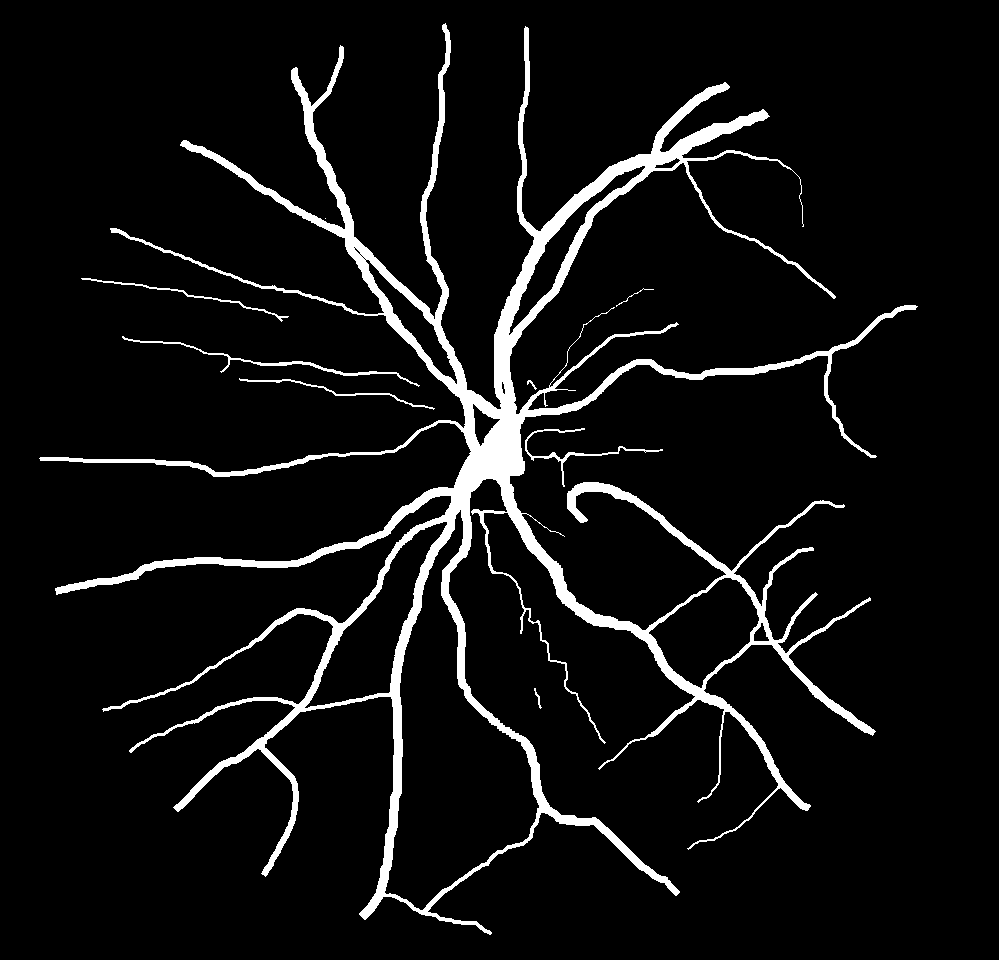
\includegraphics[width=\linewidth]{01.png}
    \caption{Ground Truth Image}
  \end{subfigure}
  \hfill
  \begin{subfigure}{0.45\textwidth}
    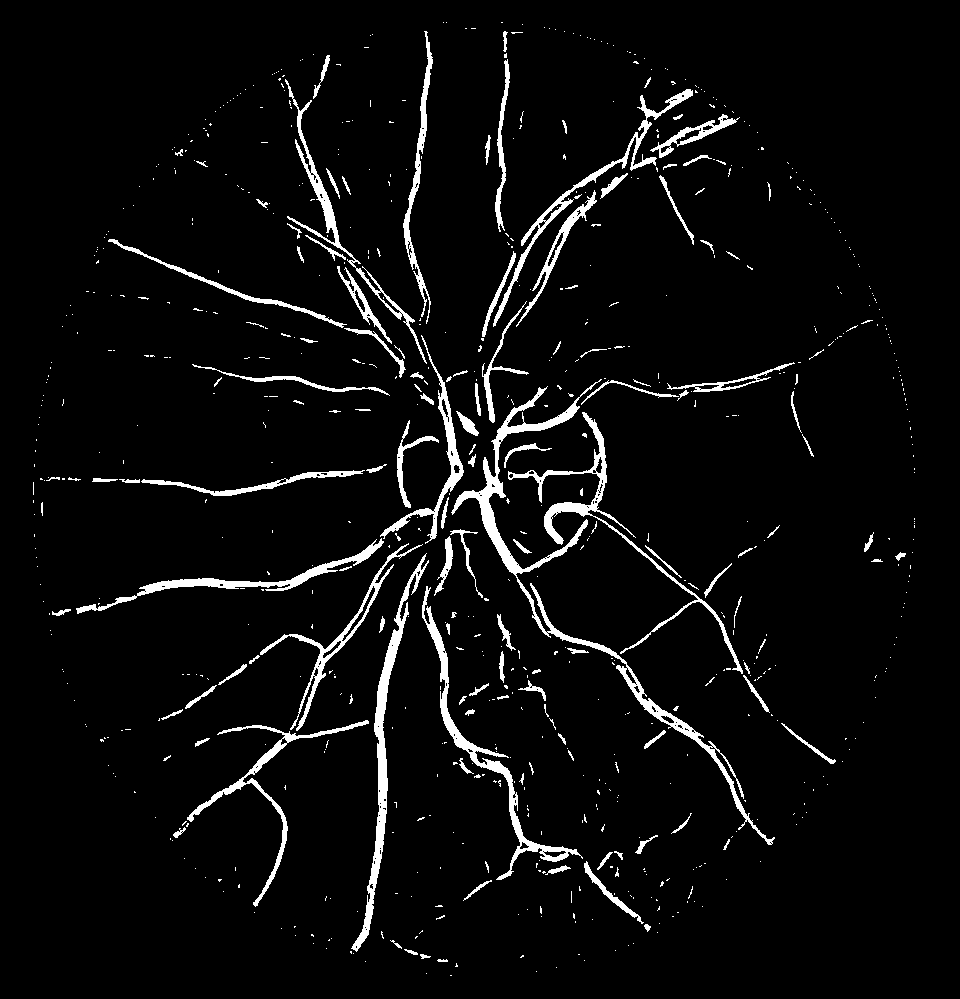
\includegraphics[width=\linewidth]{prediction1.png}
    \caption{Predicted Image}
  \end{subfigure}
  \caption{Predicted v/s Actual Image for 01L}
\end{figure}

Figure-7 shows the ground truth image and the predicted image for image 01L.jpg in the CHASEDB dataset.

\section{ Conclusion }

This report comprehensively explores the realm of medical image segmentation by underlining the methodology followed by state of the art models. Based on inferences drawn from existing research various machine learning techniques were explored to acheive best segmentation accuracy on the CHASEDB retinal image dataset. This included an unsupervised model using the KMeans clustering algorithm and a supervised model using the Random Forest Classifier. While these approaches did not give the necessary results they do warrant further research. The final approach which gave the best result was a supervised SVM model with an accuracy of 95\%. 

\section*{References}
Following are References of Articles, Research Papers and websites we used during the Phase 1 of the Project.
\medskip


{
\small


[1] A threshold based technique to extract retinal blood vessels from fundus images by Jootiprava Dash , Nilamani Bhoi

[2] Roychowdhury S, Koozekanani DD, Parhi KK. Iterative vessel segmen-
tation of fundus images. IEEE Trans Biomed Eng 2015;62(7):1738e49..

[3] Fraz MM, Basit A, Barman SA. Application of morphological bit planes
in retinal blood vessel extraction. J Digit Imaging 2013;26(2):274e86.
109

[4]https://neptune.ai/blog/data-exploration-for-image-segmentation-and-object-detection

[5]https://www.kaggle.com/code/datark1/eda-images-processing-and-exploration

[6]https://www.researchgate.net/publication/224641390\_Segmentation\_of\_Retinal\_Blood\_Vessels\_Using\_Scale-Space\_Features\_and\_K-Nearest\_Neighbour\_Classifier

[7]https://ieeexplore.ieee.org/stamp/stamp.jsp?tp\=\&arnumber\=6290653

%%%%%%%%%%%%%%%%%%%%%%%%%%%%%%%%%%%%%%%%%%%%%%%%%%%%%%%%%%%%
}

\end{document}